% !TeX spellcheck = cs_CZ
\documentclass[ 12pt, a4paper]{article}
\usepackage{lmodern}
\usepackage[utf8]{inputenc}
\usepackage[czech]{babel}
\usepackage{hyperref}
\usepackage{graphicx}
\usepackage{caption}
\usepackage{indentfirst}

\begin{document}
\def\code#1{\texttt{#1}}

\pagenumbering{gobble} %bez cisel
%
%Titulni strana
\centerline{
\includegraphics[width=12cm]{logo.png}}
\vspace*{50px}
\begin{center}
	{\LARGE\bf\noindent KIV/UIR \\ Klasifikace dokumentů}\\
	\vspace*{40px}  
	
	Tomáš Ott\\
	(A17B0314P)\\
	\vspace*{\fill}  
	\hspace*{\fill} \today \\
\end{center}
\newpage
%Obsah
\tableofcontents
\newpage



\section{Zadání}
Ve zvoleném programovacím jazyce navrhněte a implementujte program, který umožní klasifikovat textové dokumenty do tříd podle jejich obsahu, např. počasí, sport, politika, apod. Při řešení budou splněny následující podmínky:
\begin{itemize}
	
\item Použijte data z českého historického periodika Posel od Čerchova“, která jsou k dispozici na \url{https://drive.google.com/drive/folders/1mQbBNS43gWFRMHDYdSkQug47cuhPTsHJ?usp=sharing}. V původní podobě jsou data k dispozici na \url{http://www.portafontium.eu/periodical/posel-od-cerchova-1872?language=cs.}

\item Pro vyhodnocení přesnosti implementovaných algoritmů bude NUTNÉ vybrané dokumenty ručně označkovat. Každý student ručně anotuje 10 stran zadaného textu –
termín 31.3.2020. Za dodržení termínu obdrží student bonus 10b.

\item Přiřazení konkrétních textů jednotlivým studentům spolu s návodem na anotaci a příklady je uloženo spolu s daty na výše uvedené adrese, konkrétně:
	\begin{itemize}
	\item 0 - vzorová složka (takhle by měl výsledek vypadat)
	\item 1, 2, .. , 15, 101, 102, .. - data k anotaci
	\item přiřazení souboru studentum.xlsx - určení, jaké soubory má jaký student	anotovat. Až budete mít anotaci hotovou, doplňte sem informaci.
	\item Anotační příručka - návod, jak články anotovat.
	\item Klasifikace dokumentů - kategorie.xlsx - seznam kategorií k anotaci s příklady.
	\item sem prace20.pdf - Zadání semestrální práce
	\end{itemize}

\item implementujte alespoň tři různé algoritmy (z přednášek i vlastní) pro tvorbu příznaků reprezentující textový dokument.

\item implementujte alespoň dva různé klasifikační algoritmy (klasifikace s učitelem):
	\begin{itemize}
	\item Naivní Bayesův klasifikátor
	\item klasifikátor dle vlastní volby
	\end{itemize}

\item funkčnost programu bude následující:
– spuštění s parametry:\\
\textbf{název klasifikátoru, soubor se seznamem klasifikačních tříd, trénovací množina, testovací množina, parametrizační algoritmus, klasifikační algoritmus,název modelu}\\
program natrénuje klasifikátor na dané trénovací množině, použije zadaný parametrizační a klasifikační algoritmus, zároveň vyhodnotí úspěšnost klasifikace a natrénovaný model uloží do souboru pro pozdější použití (např. s GUI).– spuštění s jedním parametrem:\\
\textbf{název klasifikátoru, název modelu} \\
program se spustí s jednoduchým GUI a uloženým klasifikačním modelem. Program umožní klasifikovat dokumenty napsané v GUI pomocí klávesnice (resp. překopírované ze schránky).

\item ohodnoťte kvalitu klasifikátoru na dodaných datech, použijte metriku přesnost (accuracy), kde jako správnou klasifikaci uvažujte takovou, kde se klasifikovaná třída nachází mezi anotovanými. Otestujte všechny konfigurace klasifikátorů (tedy celkem 6 výsledků).
\end{itemize}


Poznámky:
\begin{itemize}
\item pro vlastní implementaci není potřeba čekat na dokončení anotace. Pro průběžné testování můžete použít korpus současné češtiny, který je k dispozici na \url{http://ctdc.kiv.zcu.cz/} (uvažujte pouze první třídu dokumentu podle názvu, tedy např.
dokument 05857 zdr ptr eur.txt náleží do třídy zdr“ - zdravotnictví).
”
\item další informace, např. dokumentace nebo forma odevzdávání jsou k dispozici na CW pod záložkou Samostatná práce.

\end{itemize}
\newpage
\section{Analýza zadání}

\subsection{Algoritmy pro tvorbu příznaků}
\subsubsection{Bag of words}
\subsubsection{TF-IDF}
\subsubsection{N-gram}

\subsection{Klasifikační algoritmy}
\subsubsection{Naivní Bayes}
\subsubsection{K-nejbližších sousedů}

\newpage
\section{Implementace}


\newpage
\section{Uživatelská příručka}
\subsection{Nápověda}
Vypsat nápovědu pro vstupní parametry je možné pomocí příkazu:\\
"\texttt{python Main.py -h}"\\
Zde jsou vysvětleny všechny parametry, které aplikace přijímá. Mezi ně patří:
\begin{itemize}
	\item \texttt{-c <soubor\_se\_seznamem\_klasifikacnich\_trid>} soubor, který obsahuje seznam všech tříd vyskytujících se v jednotlivých dokumentech.
	\item \texttt{-train <trenovaci\_mnozina>} množina souborů, která se využije pro naplnění příznakové struktury.
	\item \texttt{-test <testovaci\_mnozina>} množina souborů, která budou využity pro ověření funkčnosti klasifikátoru.
	\item \texttt{-p <parametrizacni\_algoritmus>} parametrizační algoritmus pomocí kterého budou reprezentovány jednotlivé dokumenty. (Pouze u trénovacího režimu) 
	\item \texttt{-k <klasifikacni\_algoritmus>} klasifikační algoritmus, který je využit pro klasifikaci dokumentů. (Pouze u trénovacího režimu)
	\item \texttt{<nazev\_modelu>} název souboru do kterého je model ukládán a v případě testovacího režimu načítán.
\end{itemize}

\subsection{Trénovací režim}
Tento režim je možné spustit zadáním následujícího příkazu:\\
"\texttt{python Main.py -c <soubor\_se\_seznamem\_klasifikacnich\_trid> 
	\\-train <trenovaci\_mnozina> -test <testovaci\_mnozina> 
	\\-p <parametrizacni\_algoritmus> -k <klasifikacni\_algoritmus> 
	\\<nazev\_modelu>}"\\

Trénovací režim neobsahuje uživatelské rozhraní a všechny jeho výstupy jsou vypisovány do terminálu. Program nejdříve naplní trénovací množinu souborů do zvolené parametrizační struktury. Poté následuje jednotlivé klasifikování testovací množiny souborů, kde jsou všechny výsledky vypsány na obrazovku. Po dokončení druhé fáze následuje vypočtení přesnosti klasifikátoru.


\subsection{Testovací režim}
Tento režim je možné spustit zadáním následujícího příkazu:\\
"\texttt{python Main.py <nazev\_modelu>}"\\
Aplikace načte předaný model díky kterému vytvoří instance klasifikátoru a struktury příznaků. Tento model je poté využíván pro klasifikaci textu zadaného uživatelem do jednoduchého uživatelského rozhraní zobrazeno na obrázku \ref{fig:screenshot001}. 

 \begin{figure}
 	\centering
 	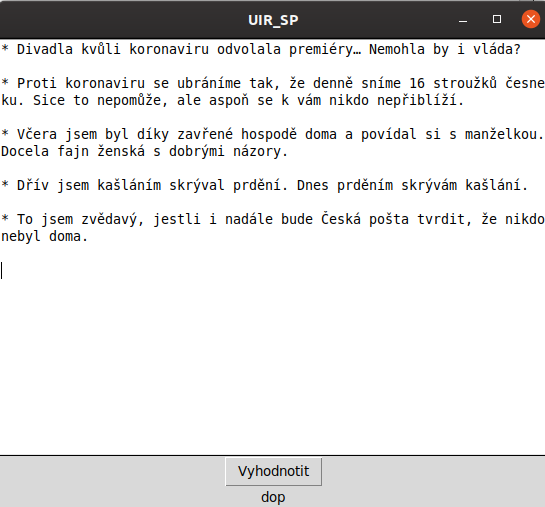
\includegraphics[width=0.7\linewidth]{screenshot001}
 	\caption{Jednoduché uživatelské rozhraní při testovacím režimu}
 	\label{fig:screenshot001}
 \end{figure}
 

\newpage
\section{Závěr}


\newpage

\end{document}